\chapter{Discriminating features for multivariate classifier training}
\label{app:bdt_features}
Figure \ref{fig:B:feature_distributions} shows the distribution of all kinematic variables chosen for histogram-based boosted decision tree training to select \demonstratorfull events.

\begin{figure}
	\centering
	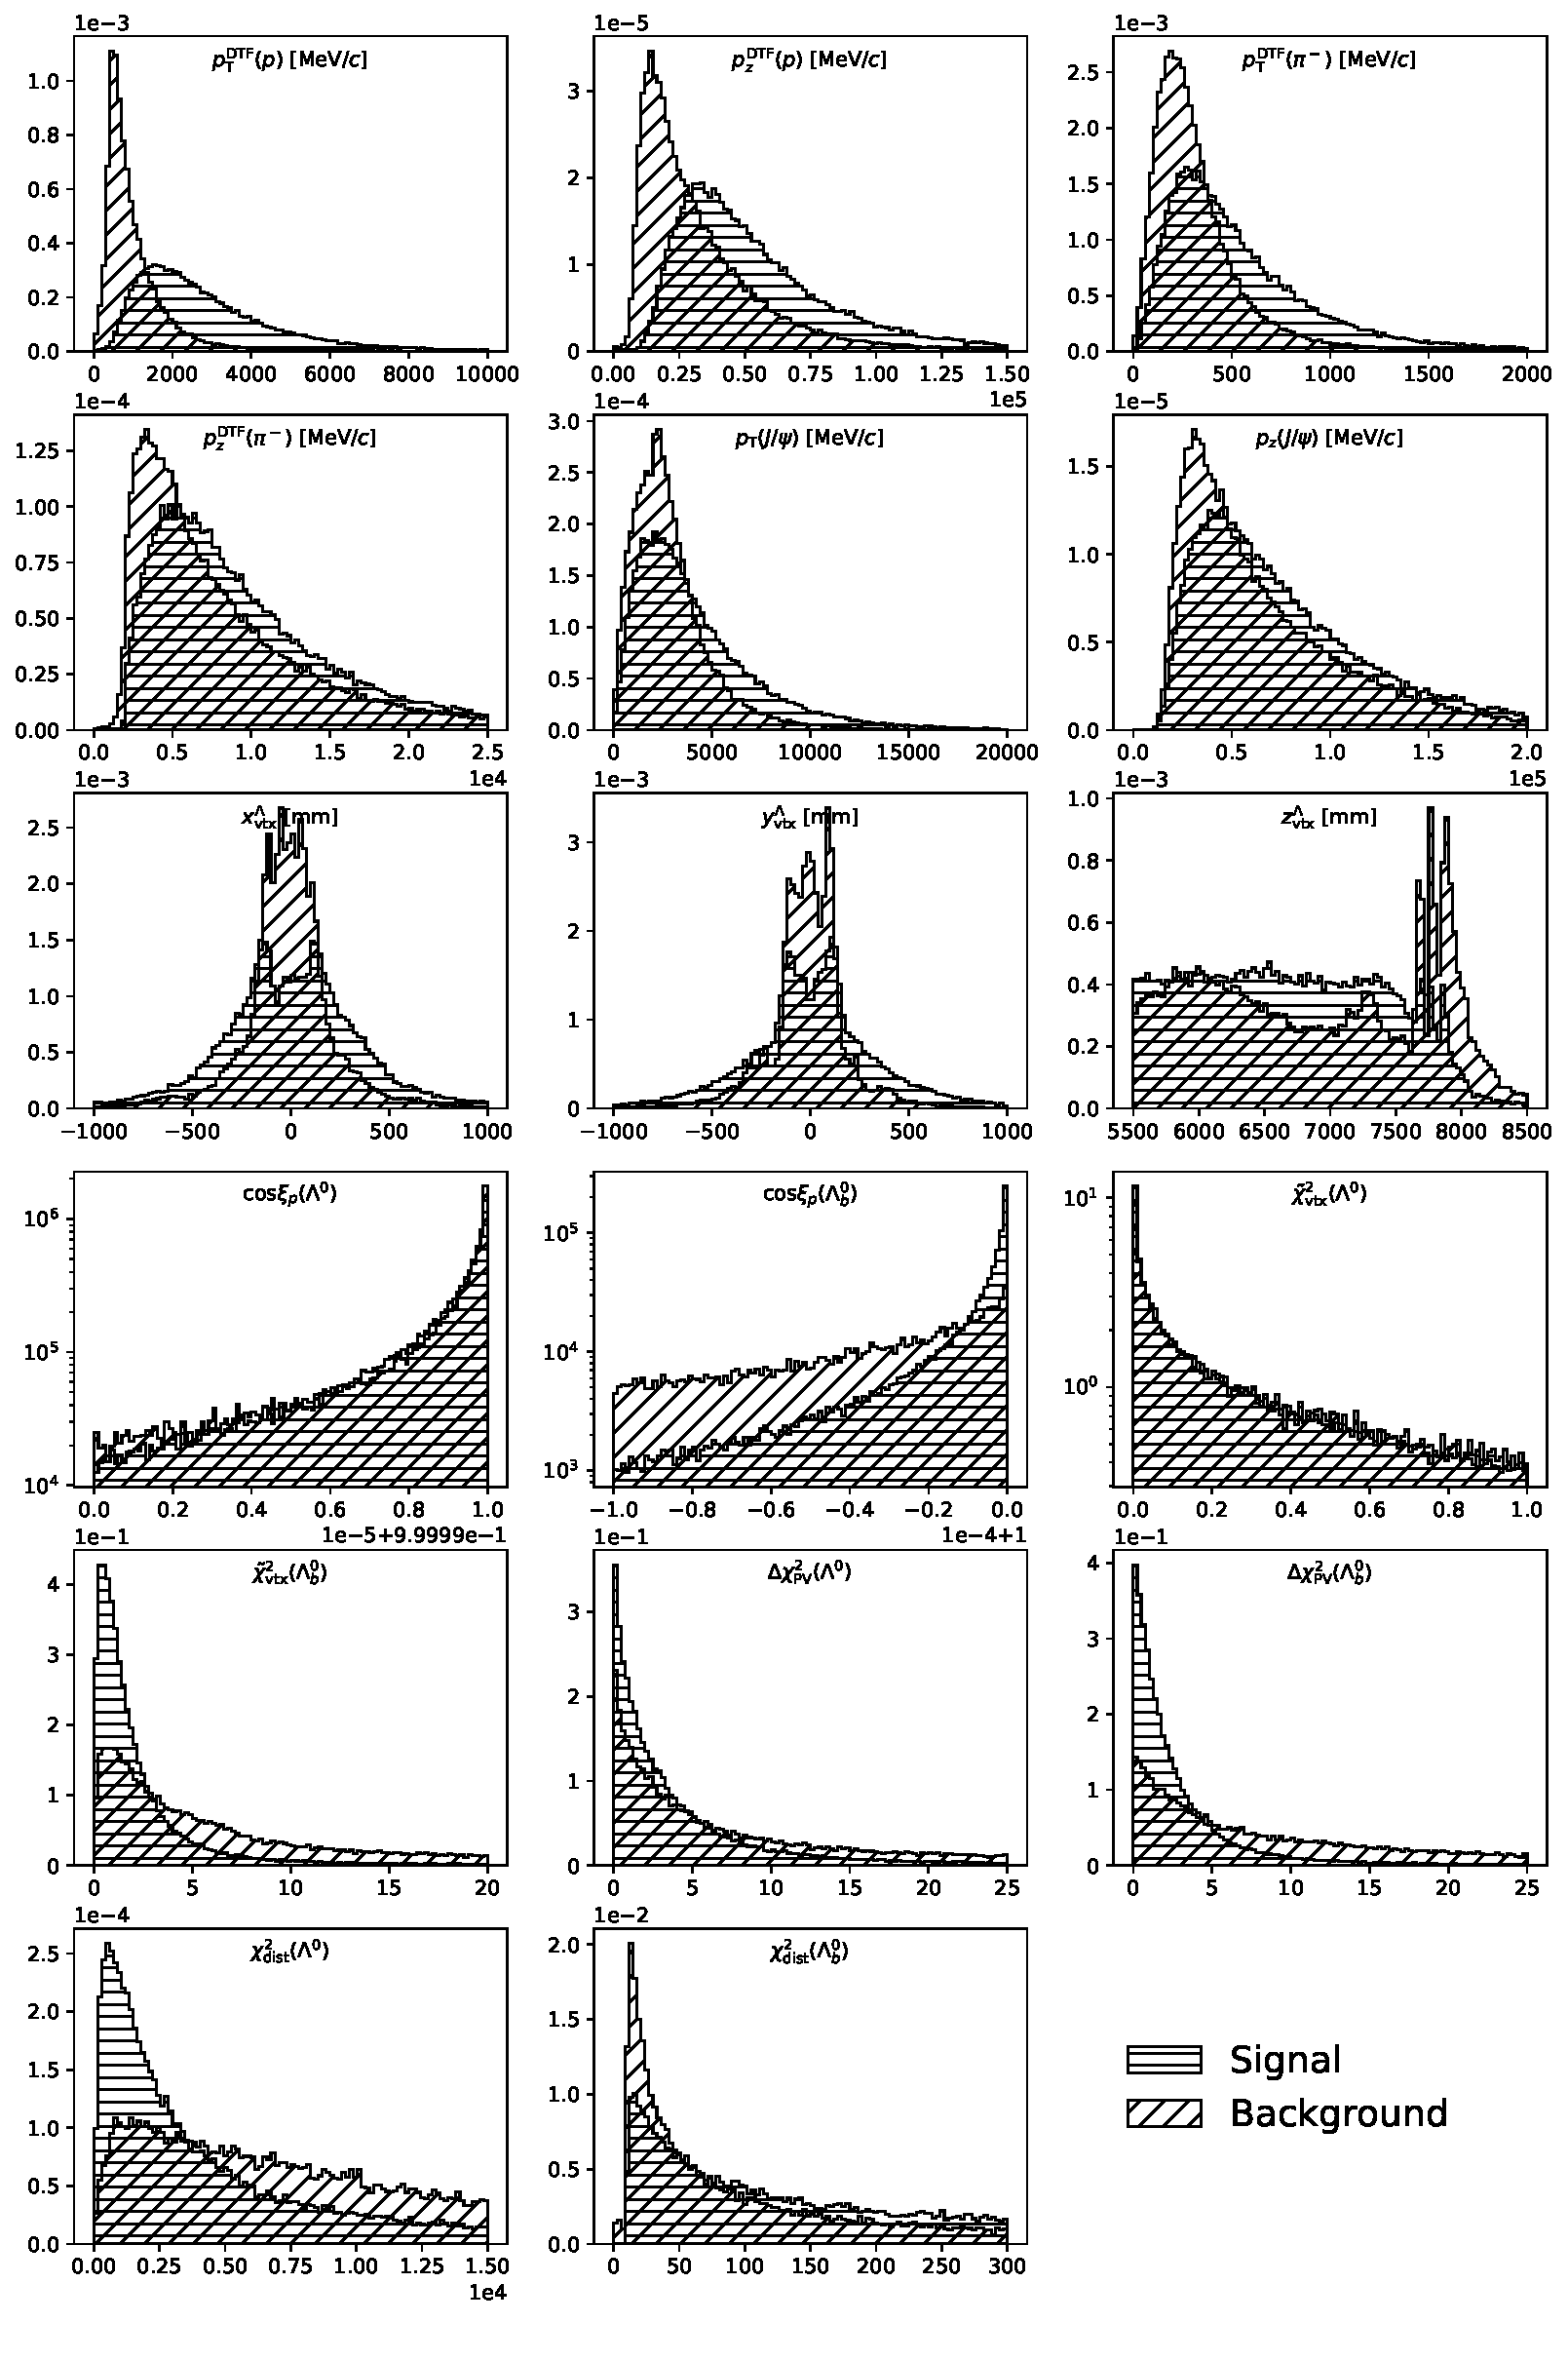
\includegraphics[width=.9\textwidth]{graphics/appendices/feature_distributions_balance.pdf}
	\caption{Normalized distributions of kinematic variables in the HBDT training data for signal (\textit{horizontal hatching}) and background from Run 2 data side bands (\textit{diagonal hatching}).
	Definitions are as in Section \ref{sec:4:train_test_data}; the $y$ axes depict probability density.}
	\label{fig:B:feature_distributions}
\end{figure}